% =====================================================================
\chapter{Materiales y métodos}\label{cap:metodos}
% =====================================================================
% Reescrito el 8 oct. 2026 segun las indicaciones de la Dra. Kruse. Fuentes:
%  - Animales: Coirini et al. 2022 (Biomedicines), seccion 2.1, traducida, mas el grupo stevia.
%  - Extracto de stevia, procedimientos conductuales, OF, SLR, inmunocitoquimica,
%    recuento celular y estadistica: borrador del laboratorio "mat meth draft".
%  - NOR: Coirini et al. 2022, seccion 2.4, traducida.
%  - SLR: texto del borrador (escrito para raton) con las medidas para rata.
% Todo lo estadistico va en la seccion de analisis estadistico, no en los demas apartados.

% ---------------------------------------------------------------------
\section{Animales de experimentación}\label{sec:diseno}

Los procedimientos con animales fueron aprobados por el Comité Institucional de Cuidado y Uso de Animales de Laboratorio (CICUAL) del Instituto de Biología y Medicina Experimental (IByME-CONICET, Argentina; protocolos 22/2020 y 18/2022), de acuerdo con los lineamientos de la Directiva del Consejo de las Comunidades Europeas (86/609/CEE) y de los Institutos Nacionales de Salud de los Estados Unidos (NIH) para el cuidado y uso de animales de laboratorio. Se utilizaron ratas macho Sprague-Dawley, alojadas en grupos de 3 a 4 animales por caja y mantenidas en un ciclo de 12\,h de luz y 12\,h de oscuridad, con alimento balanceado (Gepsa, Grupo Pilar S.A., Argentina) y agua disponibles \textit{ad libitum}.

Durante un período de 25 días, ratas de 25 días de edad (grupo juvenil) y ratas de 75 días de edad (grupo adulto) tuvieron acceso irrestricto a agua (grupos control) o la opción de beber, además de agua, una solución de sacarosa al 10\,\% (p/v; grupos sacarosa) o un extracto acuoso de \stevia{} al 4\,\% (v/v; grupos stevia) \textit{ad libitum}. Las soluciones se renovaron día por medio. Finalizado este período de 25 días de exposición, se retiraron las botellas con la solución de sacarosa o de stevia y todos los animales bebieron únicamente agua durante otros 25 días (Figura~\ref{fig:linea-temporal}) \cite{kruse2019sucrose,coirini2022sucrose}. Al finalizar el protocolo, los animales fueron evaluados en las pruebas conductuales: \textit{open field} (OF), reconocimiento de objeto novedoso (NOR) y reconocimiento espontáneo de posición (SLR). Luego de las pruebas, un subgrupo de animales de cada grupo fue perfundido para los estudios de inmunocitoquímica (\S\ref{sec:histologia}). El número de animales por grupo en cada prueba se indica en el Capítulo~\ref{cap:resultados} y, para la SLR, en el \ref{anx:muestra}.

El consumo de agua, de solución endulzada (sacarosa o stevia) y de alimento se registró día por medio durante todo el período experimental, y el peso corporal, una vez por semana. El consumo se midió por caja y se normalizó al peso corporal total de los animales alojados en ella (mL o g por g de peso corporal por día); por lo tanto, la caja se consideró la unidad experimental en todos los análisis de consumo. Como medida de la preferencia por la solución endulzada se calculó el cociente entre el volumen de solución endulzada y el volumen total de líquido ingerido durante el tratamiento.

\begin{figure}[htbp]
\centering
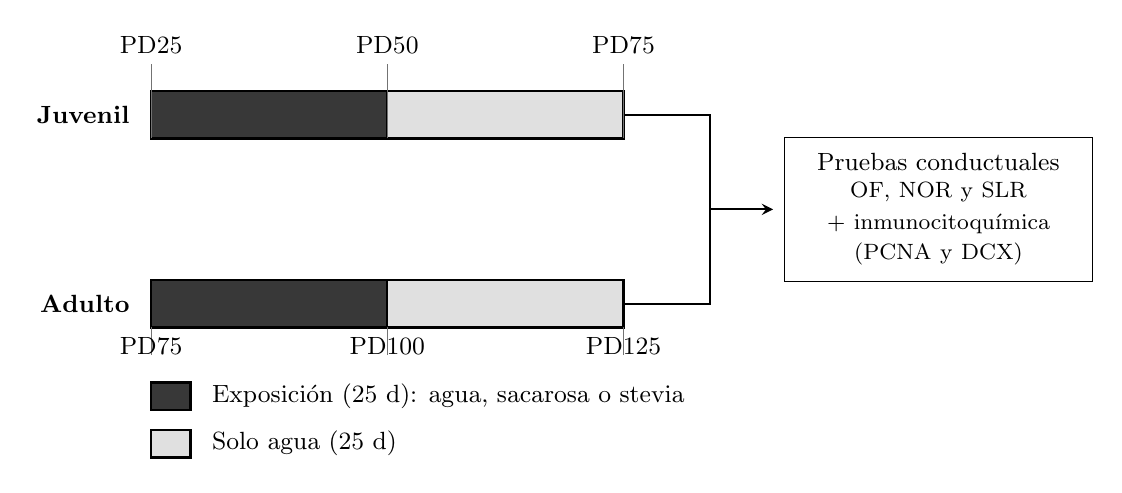
\begin{tikzpicture}[
    font=\small,
    >=stealth,
    line/.style={draw, black, thick},
    dayline/.style={draw, black!55, thin},
  ]
  % ---- fila juvenil ----
  \node[anchor=east] at (-0.15,2.7) {\textbf{Juvenil}};
  \fill[black!78] (0,2.4) rectangle (3,3.0);
  \fill[black!12] (3,2.4) rectangle (6,3.0);
  \draw[line] (0,2.4) rectangle (6,3.0);
  \draw[line] (3,2.4) -- (3,3.0);
  \foreach \x/\lbl in {0/PD25, 3/PD50, 6/PD75}
    \draw[dayline] (\x,2.4) -- (\x,3.35) node[above, black] {\lbl};

  % ---- fila adulta ----
  \node[anchor=east] at (-0.15,0.3) {\textbf{Adulto}};
  \fill[black!78] (0,0.0) rectangle (3,0.6);
  \fill[black!12] (3,0.0) rectangle (6,0.6);
  \draw[line] (0,0.0) rectangle (6,0.6);
  \draw[line] (3,0.0) -- (3,0.6);
  \foreach \x/\lbl in {0/PD75, 3/PD100, 6/PD125}
    \draw[dayline] (\x,-0.35) -- (\x,0.0) node[below, black] {\lbl};

  % ---- convergencia hacia el desenlace común ----
  \draw[black, thick] (6,2.7) -- (7.1,2.7) -- (7.1,0.3) -- (6,0.3);
  \draw[black, thick, ->] (7.1,1.5) -- (7.9,1.5);
  \node[draw=black, align=center, fill=white, text width=3.5cm, inner sep=6pt] at (10.0,1.5)
    {Pruebas conductuales\\ \footnotesize OF, NOR y SLR\\[2pt] + inmunocitoquímica\\ \footnotesize (PCNA y DCX)};

  % ---- leyenda (apilada) ----
  \fill[black!78] (0,-1.05) rectangle (0.5,-0.7);
  \draw[line] (0,-1.05) rectangle (0.5,-0.7);
  \node[anchor=west] at (0.65,-0.875) {Exposición (25 d): agua, sacarosa o stevia};
  \fill[black!12] (0,-1.65) rectangle (0.5,-1.3);
  \draw[line] (0,-1.65) rectangle (0.5,-1.3);
  \node[anchor=west] at (0.65,-1.475) {Solo agua (25 d)};
\end{tikzpicture}
\caption[Línea temporal de los procedimientos experimentales]{Línea temporal de los procedimientos experimentales. Durante 25 días, ratas de 25 días de edad (grupo juvenil) y de 75 días de edad (grupo adulto) tuvieron acceso irrestricto a agua (control) o la opción de beber, además de agua, una solución de sacarosa al 10\,\% o un extracto de stevia al 4\,\%. Luego, todos los animales bebieron únicamente agua durante otros 25 días, tras lo cual se realizaron las pruebas conductuales y los estudios de inmunocitoquímica. PD: día postnatal.}
\label{fig:linea-temporal}
\end{figure}

% ---------------------------------------------------------------------
\section{Preparación y caracterización de la infusión de stevia}\label{sec:soluciones}

Las hojas de \stevia{} se obtuvieron de Caña Dulce\textsuperscript{\textregistered} (San Ignacio, Misiones, Argentina), con certificación de Argencert, Argentina (R.P.A.A. N.º~MI000348 y R.P.E.A. N.º~MI000097). El extracto de stevia se preparó según un método descrito previamente \cite{kruse2025stevia}, adaptado de Sharma et~al.\ \cite{sharma2009stevia}, elegido por su alto rendimiento de glucósidos de esteviol \cite{celaya2022infusions} y por su similitud con los procedimientos de preparación orientados a la salud. Se hirvieron 20\,g de hojas de stevia en 1\,L de agua durante 10\,min, se dejó reposar 20\,min, se filtró y se volvió a hervir durante 45--50\,min hasta reducir el volumen a 300\,mL. El extracto se fraccionó en alícuotas de 40\,mL, que se almacenaron a \SI{-20}{\celsius}; las alícuotas se descongelaron día por medio y se diluyeron a 1\,L (4\,\% v/v). La solución de sacarosa al 10\,\% (p/v; Ledesma, Argentina) se preparó en agua. Estas concentraciones se eligieron sobre la base de estudios previos y del consumo voluntario de los animales \cite{coirini2022sucrose,rey2024metformin,kruse2019sucrose,kruse2025stevia}.

La caracterización química del extracto de stevia fue realizada por el Laboratorio Central de la Facultad de Ciencias Exactas, Químicas y Naturales (FCEQyN) de la Universidad Nacional de Misiones (Argentina), siguiendo protocolos establecidos \cite{yildizozturk2015extraction,celaya2022infusions}. El contenido de glucósidos de esteviol se determinó por cromatografía líquida de alta eficacia (HPLC) con una columna amino. Los compuestos fenólicos totales y los taninos se cuantificaron con un espectrofotocolorímetro y se expresaron como miligramos equivalentes de ácido gálico (GAE) por mililitro de extracto, y el contenido de flavonoides, como miligramos equivalentes de quercetina (QE) por mililitro. La actividad antioxidante se evaluó mediante el ensayo de captación del radical 2,2-difenil-1-picrilhidrazilo (DPPH), con quercetina como estándar de referencia (IC$_{50}$ = $4{,}35 \pm 0{,}21$\,\si{\micro\gram}/mL). La composición del extracto se resume en la Tabla~\ref{tab:extracto}.

\begin{table}[htbp]
\centering
\caption[Composición química del extracto de stevia]{Composición química del extracto de stevia. Los valores se expresan como media $\pm$ SEM ($n = 3$). DPPH: 2,2-difenil-1-picrilhidrazilo; GAE: equivalentes de ácido gálico; QE: equivalentes de quercetina; IC$_{50}$: concentración inhibitoria media.}
\label{tab:extracto}
\small
\begin{tabular}{@{}l l@{}}
\toprule
\textbf{Componente} & \textbf{Valor} \\
\midrule
Esteviósido & $3{,}80 \pm 0{,}29$\,mg/mL \\
Rebaudiósido A & $1{,}47 \pm 0{,}10$\,mg/mL \\
Rebaudiósido C & $0{,}25 \pm 0{,}02$\,mg/mL \\
Glucósidos de esteviol totales & $5{,}52 \pm 0{,}42$\,mg/mL \\
Fenoles & $2{,}99 \pm 0{,}38$\,mg GAE/mL de extracto \\
Flavonoides & $1{,}49 \pm 0{,}17$\,mg QE/mL de extracto \\
Taninos & $1{,}73 \pm 0{,}11$\,mg GAE/mL de extracto \\
Actividad antioxidante (DPPH), IC$_{50}$ & $14{,}04 \pm 0{,}56$\,\si{\micro\gram}/mL \\
\bottomrule
\end{tabular}
\end{table}

% ---------------------------------------------------------------------
\section{Procedimientos conductuales}\label{sec:conductual}

Los dispositivos de prueba se iluminaron con una luz de 42\,W suspendida a aproximadamente 1\,m de altura y dirigida hacia el techo. Los animales se aclimataron a la sala de comportamiento durante 20\,min antes de las pruebas, que se realizaron por la mañana (10:00\,h). Los dispositivos se limpiaron con etanol al 70\,\% entre animales. Las sesiones de comportamiento se grabaron en video, se codificaron y se analizaron con el software de seguimiento \anymaze{} (Stoelting Co., EE.\,UU.).

\subsection{\textit{Open field} (OF)}\label{sec:of}

El dispositivo consistió en una arena cuadrada de 75\,cm de lado con paredes opacas de 30\,cm de alto. Las ratas se colocaron en el centro de la arena y se les permitió explorarla libremente durante 5\,min. La arena se dividió digitalmente en tres zonas concéntricas: central, intermedia y periférica (zonas 1 a 3; Figura~\ref{fig:of-esquema}). El piso de la arena está dividido en una cuadrícula de $5 \times 5$ cuadrados de 15\,cm de lado: la zona 1 corresponde al cuadrado central ($15 \times 15$\,cm); la zona 2, al anillo de ocho cuadrados que lo rodea (límite externo de $45 \times 45$\,cm); y la zona 3, a la franja de 15\,cm de ancho adyacente a las paredes. Se registraron la distancia total recorrida, el número de zonas visitadas y las entradas, las distancias recorridas y el tiempo de permanencia en cada zona \cite{kruse2019sucrose}. Se registró además el \textit{rearing}, una conducta de exploración vertical en la que el animal se incorpora sobre las patas traseras \cite{lever2006rearing}, como número de eventos y tiempo total.

\begin{figure}[htbp]
  \centering
  \incluirfigura[width=0.4\linewidth]{Fig4_OF_zonas.png}
  \caption[Aparato de \textit{open field} (OF) y zonas de registro]{Aparato de \textit{open field} (OF) y zonas de registro: captura cenital de \anymaze{} de la arena (75\,cm de lado), con la cuadrícula del piso (cuadrados de 15\,cm de lado) y las tres zonas definidas digitalmente: central (1), intermedia (2) y periférica (3).}
  \label{fig:of-esquema}
\end{figure}

\subsection{Reconocimiento de objeto novedoso (NOR)}\label{sec:nor}

El aparato consistió en una caja abierta de madera oscura (75\,cm de largo $\times$ 30\,cm de alto $\times$ 55\,cm de ancho), iluminada por una luz de 42\,W suspendida a 100\,cm por encima de la caja y dirigida hacia el techo. La intensidad de la luz fue igual en las distintas partes del aparato. Los objetos a discriminar diferían en forma y textura; eran de vidrio, plástico, cerámica o metal y tenían cuatro formas distintas (frascos de vidrio, tazas de cerámica, cilindros metálicos y cubos de plástico), y no podían ser desplazados por las ratas \cite{perezgarcia2016malnutrition,leger2013nor}. Brevemente, durante la semana previa a la prueba las ratas fueron manipuladas una vez al día durante 3 días consecutivos. Cinco días antes de la prueba se permitió que las ratas exploraran el aparato durante 6\,min por día. En estas sesiones de habituación no había objetos en la caja. Veinticuatro horas después de la última sesión de habituación, las ratas fueron entrenadas para el reconocimiento de objetos permitiéndoles explorar durante 6\,min dos objetos idénticos colocados en la arena de prueba (fase de muestreo). Durante esta fase de muestreo (T1), los objetos (dos frascos de vidrio de 12,5\,cm de alto y 5\,cm de diámetro) se colocaron al azar en dos esquinas opuestas del aparato, a 10\,cm de las paredes laterales (Figura~\ref{fig:nor-objetos}A). La rata se colocó en el centro del aparato y se le permitió explorar los dos objetos idénticos. Después de T1, la rata fue devuelta a su caja y, tras un intervalo entre ensayos de 2\,h (memoria a corto plazo, T2), de 24\,h (memoria a largo plazo, T3) y de 7 días desde la fase de muestreo (memoria consolidada, T4), fue evaluada nuevamente en los ensayos de elección. Durante T2, T3 y T4, un objeto novedoso reemplazó a uno de los objetos presentados durante T1. Así, las ratas fueron reexpuestas durante 6\,min a dos objetos: una copia del objeto familiar (F) y el objeto novedoso (N) (Figura~\ref{fig:nor-objetos}B); es decir, un frasco de vidrio se reemplazó por un cilindro metálico amarillo y rugoso de 9,5\,cm de alto y 5,5\,cm de diámetro, por una caja de plástico anaranjada de 10,5\,cm de largo $\times$ 9\,cm de ancho $\times$ 4\,cm de alto y por una taza cónica de cerámica blanca de 8,5\,cm de alto y 8,5\,cm de diámetro en T2, T3 y T4, respectivamente. Todas las combinaciones y ubicaciones de los objetos se contrabalancearon para reducir el posible sesgo causado por la preferencia por ubicaciones u objetos particulares. Las sesiones T1 a T4 se grabaron en video y se analizaron los cruces de línea con el software \anymaze{} (Stoelting Co., Wood Dale, IL, EE.\,UU.). El tiempo que las ratas dedicaron a explorar cada objeto durante T1 a T4 fue registrado manualmente por un único experimentador que desconocía la asignación de los grupos. La exploración se definió de la siguiente manera: dirigir la nariz hacia el objeto a una distancia de 2\,cm o menos y/o tocar el objeto con la nariz. Dar vueltas alrededor del objeto o sentarse sobre él no se consideró comportamiento exploratorio. Los datos se informan como la tasa de exploración, que es el tiempo dedicado a explorar el objeto novedoso ($t_N$) dividido por el tiempo dedicado a explorar ambos objetos:
\begin{equation}
  \text{tasa de exploración} = \frac{t_N}{t_N + t_F}.
  \label{eq:tasa}
\end{equation}

\begin{figure}[htbp]
  \centering
  \begin{subfigure}[b]{0.38\linewidth}
    \centering
    \incluirfigura[width=\linewidth]{Fig4_NOR_objetos_iguales.png}
    \caption{}
  \end{subfigure}
  \hspace{1.5em}
  \begin{subfigure}[b]{0.38\linewidth}
    \centering
    \incluirfigura[width=\linewidth]{Fig4_NOR_objetos_diferentes.png}
    \caption{}
  \end{subfigure}
  \caption[Fases del NOR]{Fases del NOR en vista cenital. (A)~Fase de muestreo (T1): dos objetos idénticos. (B)~Ensayos de elección (T2 a T4): una copia del objeto familiar y un objeto novedoso.}
  \label{fig:nor-objetos}
\end{figure}

\subsection{Reconocimiento espontáneo de posición (SLR)}\label{sec:slr}

Este procedimiento se realizó como fue descrito por Reichelt et~al.\ \cite{reichelt2016sucrose,reichelt2021slr}. El aparato consistió en un campo abierto circular de plástico gris y base opaca, de 100\,cm de diámetro $\times$ 45\,cm de alto, sin techo. Una cámara de video colocada por encima del dispositivo grabó cada sesión. La arena estuvo rodeada de tres señales espaciales distintivas (pósteres negros y blancos con patrones únicos) de 35\,cm de alto $\times$ 50\,cm de ancho, ubicadas equidistantes alrededor de la arena, y de las señales distales proporcionadas por los muebles de la sala, incluidos los estantes y la puerta.

Durante la semana previa a la habituación, los animales fueron manipulados una vez al día durante 5 días consecutivos. Antes del día del primer ensayo se permitió que cada animal explorara el dispositivo durante 10\,min por día durante 3 días consecutivos (habituación). Los objetos fueron tazas con dibujos o ranas de juguete (Figura~\ref{fig:objetos-slr}), limpiados con etanol al 70\,\% entre pruebas; dentro de cada sesión, los objetos de la fase de muestreo y de la fase de prueba fueron copias idénticas.

En el primer ensayo se expuso a las ratas a tres objetos idénticos, A1, A2 y A3, durante 10\,min (fase de muestreo). La disposición de los objetos dependió de la configuración evaluada: d-SLR o s-SLR (Figura~\ref{fig:esquema-slr}). En ambas configuraciones, los objetos se colocaron a lo largo de una circunferencia, a 10\,cm de la pared, aproximadamente. En cada experimento, la mitad de los animales fue asignada a la tarea d-SLR y la otra mitad a la s-SLR ($n$ = 9--10 por grupo y configuración; \ref{anx:muestra}). Para la d-SLR, los objetos A1, A2 y A3 se colocaron equidistantes, a 120° y a una distancia aproximada de 49\,cm entre ellos. Para la s-SLR, los objetos A2 y A3 se colocaron a 50° de distancia, a 20,5\,cm entre ellos, mientras que A1 se ubicó a la misma distancia de A2 y de A3. La demanda de separación de patrones es mayor cuanto menor es la distancia entre los objetos, de modo que la s-SLR impone una demanda cognitiva mayor que la d-SLR \cite{reichelt2021slr}. Veinticuatro horas después de la fase de muestreo, los animales regresaron a la arena, donde fueron expuestos solo a dos objetos, uno familiar (A1) y otro novedoso (N), durante 5\,min (fase de prueba). El objeto N se ubicó en la posición media entre las que ocupaban los objetos A2 y A3 en la fase de muestreo.

\begin{figure}[htbp]
  \centering
  \incluirfigura[width=0.9\linewidth]{Fig4_esquema_SLR.png}
  \caption[Esquema de la prueba de reconocimiento espontáneo de posición (SLR)]{Esquema de la prueba de reconocimiento espontáneo de posición (SLR). En la fase de muestreo (día 1, 10\,min) el animal explora tres objetos idénticos (A1, A2 y A3) en la configuración d-SLR (fila superior) o s-SLR (fila inferior). En la fase de prueba (día 2, 24\,h después, 5\,min) se presentan dos objetos: uno en la posición familiar de A1 y otro en una posición novedosa (N), ubicada entre las posiciones que antes ocupaban A2 y A3 (círculos punteados). Los símbolos oscuros alrededor de la arena representan las señales espaciales. Adaptado de \cite{reichelt2021slr}.}
  \label{fig:esquema-slr}
\end{figure}

\begin{figure}[htbp]
  \centering
  \incluirfigura[width=0.7\linewidth]{Fig4_objetos_SLR.jpg}
  \caption{Objetos utilizados en la prueba SLR: tazas con dibujos y ranas de juguete.}
  \label{fig:objetos-slr}
\end{figure}

\textbf{Análisis de comportamiento.} La exploración se definió de la siguiente manera: dirigir la nariz hacia el objeto a una distancia de 2\,cm o menos y/o tocar el objeto con la nariz y las vibrisas moviéndose alrededor del objeto. Dar la vuelta o sentarse sobre el objeto no se consideró comportamiento exploratorio. El tiempo empleado por las ratas en explorar cada objeto fue cronometrado manualmente por un único observador que desconocía la asignación de los grupos. Los datos se informan como el índice de discriminación (DI), que es la diferencia entre el tiempo dedicado a explorar el objeto en la posición novedosa ($t_N$) y el tiempo de exploración del objeto en la posición familiar ($t_F$), dividida por el tiempo total de exploración de ambos objetos:
\begin{equation}
  \mathrm{DI} = \frac{t_N - t_F}{t_N + t_F}.
  \label{eq:di}
\end{equation}
Se informa también la tasa de exploración equivalente (Ecuación~\ref{eq:tasa}), de la cual el DI es una transformación lineal ($\mathrm{DI} = 2\cdot\text{tasa} - 1$). Como control, se midió la locomoción de las ratas en la arena mediante el software de seguimiento \anymaze{} (Stoelting Co., EE.\,UU.).

\subsection{Registro con \anymaze}\label{sec:principio}

El seguimiento se realizó con \anymaze{} (versión 7.66) sobre el video cenital de cada sesión. El programa registra de forma automática la posición del animal y, a partir de ella, calcula la distancia recorrida, los cruces de línea y las entradas, la distancia y el tiempo de permanencia en las zonas definidas por el usuario. La exploración de los objetos en el NOR y en la SLR y el \textit{rearing} en el OF no se obtuvieron del seguimiento automático: se puntuaron de forma manual sobre las sesiones grabadas, como se describió para cada prueba.

% ---------------------------------------------------------------------
\section{Inmunocitoquímica y microscopía de fluorescencia}\label{sec:histologia}

Los animales \confirmar{número de animales por grupo: el borrador del laboratorio indica $n = 4$ en este apartado y $n = 6$ en el de animales} fueron anestesiados profundamente mediante una inyección intraperitoneal de hidrato de cloral al 28\,\% (p/v; 0,1\,mL/100\,g de peso corporal) y fijados por perfusión intracardíaca con 600\,mL de paraformaldehído (PFA) al 4\,\% frío en PBS (pH~7,4) \cite{kruse2012lxr}. Los cerebros se extrajeron de inmediato y se dejaron en PFA al 4\,\% durante toda la noche a \SI{4}{\celsius}. Luego se lavaron con PBS y se seccionaron con un vibrátomo. Se obtuvieron cortes coronales de \SI{70}{\micro\metre} de espesor (Bregma $-2{,}8$ a $-4{,}2$\,mm), determinados con un atlas del cerebro de rata \cite{paxinos1986rat}, que se incubaron en PBS con 0,1\,\% de Tween~20 y 7\,\% de suero normal de burro durante 1\,h a temperatura ambiente. Las muestras de tejido se incubaron luego con un anticuerpo de ratón anti-PCNA (dilución 1:250; ref.\ MAB424, Merck) y un anticuerpo de cabra anti-DCX (dilución 1:200; ref.\ sc-8066, Santa Cruz Biotechnology) en PBS con 2\,\% de suero de burro y 0,1\,\% de Tween~20, durante toda la noche a \SI{4}{\celsius}. Posteriormente se lavaron en PBS durante 30\,min y se incubaron con un anticuerpo de burro anti-ratón Alexa~488 y un anticuerpo de burro anti-cabra Alexa~555 (ref.\ A21202 y A21432, respectivamente; Thermo Fisher; ambos en dilución 1:1000) durante 2\,h a temperatura ambiente. Los núcleos se contratiñeron con DAPI (1\,\si{\micro\gram}/mL). Finalmente, después de los lavados, los cortes se montaron en portaobjetos de vidrio y se examinaron con un microscopio confocal de disco giratorio Olympus IX81-DSU. Todas las imágenes se obtuvieron en las mismas condiciones: el tiempo de exposición, la intensidad de la lámpara y los filtros se mantuvieron constantes. En algunos cortes se omitió el anticuerpo primario como control; estos cortes se procesaron con el mismo protocolo descrito, y la intensidad de fluorescencia obtenida en ellos se utilizó como referencia para identificar la marca positiva. Todos los portaobjetos se codificaron y fueron analizados por dos observadores independientes que desconocían el tratamiento.

\begin{figure}[htbp]
  \centering
  \incluirfigura[width=0.85\linewidth]{Fig4_confocal_giro_dentado.png}
  \caption[Fotomicrografías confocales del giro dentado (PCNA y DCX)]{Fotomicrografías confocales representativas del giro dentado. \pendiente{Insertar foto: panel con una imagen por marcador (PCNA y DCX) y DAPI de un mismo animal control, más una imagen combinada; barra de escala y aumento del objetivo indicados.}}
  \label{fig:confocal-giro-dentado}
\end{figure}

\subsection{Recuento celular}\label{sec:recuento}

Los cortes se tomaron en una serie 1:4 (separados por \SI{280}{\micro\metre}; 5 cortes por animal) \confirmar{número de cortes por animal: el borrador del laboratorio indica 5 en este apartado y 3 secciones por región en el de animales} y se analizaron con ImageJ Fiji win64 (\url{http://imagej.nih.gov/ij}). Las células positivas para PCNA y/o DCX se contaron dentro de un área delimitada que comprendía la zona subgranular del giro dentado. Para el recuento se consideraron tanto la hoja superior como la inferior de la capa de células granulares y de la zona subgranular. El número de células inmunopositivas fue contado manualmente por dos observadores independientes que desconocían el protocolo experimental. Los resultados se expresan como número de células positivas por mm$^2$.

% ---------------------------------------------------------------------
\section{Análisis estadístico}\label{sec:estadistico}

El tamaño muestral se estimó sobre la base de estudios previos (95\,\% de confianza, 10\,\% de error, 80\,\% de potencia) \cite{coirini2022sucrose,rey2024metformin,kruse2019sucrose,kruse2025stevia}, siguiendo las recomendaciones habituales \cite{charan2013sample}. La normalidad y la homogeneidad de varianzas se evaluaron mediante las pruebas de Shapiro-Wilk y de Brown-Forsythe, respectivamente.

El consumo de líquidos durante el tratamiento se analizó mediante ANOVA de medidas repetidas, con la edad y el tratamiento como factores entre sujetos y el fluido y el tiempo como factores intrasujeto; el consumo de agua durante el período posterior al tratamiento, mediante ANOVA de medidas repetidas (edad, tratamiento y tiempo); y el curso temporal del consumo de alimento dentro de cada edad, mediante ANOVA de medidas repetidas (tratamiento y tiempo). En los tres casos se aplicó la corrección de Geisser-Greenhouse. El consumo promedio de alimento del período se analizó mediante ANOVA de dos vías (edad $\times$ tratamiento). En los análisis de consumo, las comparaciones múltiples se realizaron con la prueba de Šídák.

Las variables del OF, la tasa de exploración del NOR (T2, T3 y T4 por separado) y el DI y la tasa de exploración de la SLR (d-SLR y s-SLR por separado) se analizaron mediante ANOVA de dos vías (edad $\times$ tratamiento). Cuando se detectaron efectos significativos, se aplicó la prueba \textit{post hoc} de Tukey para ajustar por comparaciones múltiples y controlar la tasa de error por familia: en el OF se compararon los tres tratamientos dentro de cada edad, y en el NOR y la SLR, la media de cada grupo con las de su misma edad y las de su mismo tratamiento. Además, la tasa de exploración del NOR y el DI de la SLR de cada grupo se compararon con el nivel de azar (0,5 y 0, respectivamente) mediante la prueba $t$ de una muestra; valores por encima del azar indican preferencia por el objeto o la posición novedosos. Dado que el DI es una transformación lineal de la tasa de exploración, ambos índices producen resultados estadísticos idénticos. Los valores negativos del DI se consideraron válidos y no se corrigieron ni se excluyeron. Cuando los residuos se apartaron de la normalidad, las diferencias significativas se confirmaron con la prueba no paramétrica de Mann-Whitney. La exploración total de los objetos en la SLR (fase de muestreo y fase de prueba) se analizó mediante ANOVA de dos vías (edad $\times$ tratamiento) sobre el logaritmo del tiempo, seguido de la prueba de Tukey. Los marcadores de inmunocitoquímica (PCNA y DCX) se analizaron mediante ANOVA de una vía seguido de la prueba de Tukey.

La significancia estadística se estableció en $p < 0{,}05$ y los datos se expresan como media $\pm$ SEM. Las diferencias de medias se informan como primer grupo menos segundo grupo, en el orden en que ambos se nombran en cada comparación. Los datos provienen de cohortes experimentales independientes, realizadas en distintos momentos con grupos independientes de animales pero siguiendo el mismo diseño y los mismos protocolos (el OF y el NOR, en cohortes anteriores a 2026; la SLR, en cohortes de 2024 a 2026, con los grupos control provenientes de las cohortes de 2025). Los datos de las cohortes se combinaron para el análisis estadístico, sin evaluar previamente un efecto de cohorte, lo que se considera una limitación (\S\ref{sec:disc-limitaciones}). Los valores extremadamente atípicos se excluyeron del análisis; en la SLR no se excluyó ningún valor. Los análisis se realizaron con GraphPad Prism 11.1.0, salvo el de la exploración total de la SLR, que se calculó en Python (statsmodels y SciPy).

% ---------------------------------------------------------------------
\section{Análisis multivariado y aprendizaje automático}\label{sec:ml}

De manera complementaria al análisis univariado, y por las razones formales expuestas en \S\ref{sec:multivariado}, el conjunto de métricas conductuales extraídas con \anymaze{} se sometió a un análisis multivariado. Se aplicó análisis de componentes principales (PCA) sobre las variables estandarizadas para reducir la dimensionalidad y mitigar la colinealidad, seguido de clustering jerárquico con criterio de Ward sobre las puntuaciones retenidas, a fin de examinar la emergencia de perfiles conductuales sin supervisión (objetivo M1). Para el objetivo M2 se entrenó un clasificador de Random Forest con las métricas conductuales como predictores del grupo de exposición, estimando el error de generalización por validación \textit{out-of-bag} y la importancia relativa de cada variable por disminución media de impureza y por permutación. El \textit{pipeline} se implementó en Python con la biblioteca scikit-learn.
